\subsection{Adding Damped Backgrounds}
    \begin{frame}{Implementation | Adding Damped Distribution}
        .{\bf WHAT DISTRIBUTIONS TO CONSIDER...}
        
        Tried to be as general here as possible:
        \begin{itemize}
            \item  Consider arbitrary ``damping'' as a map on particle speeds
            \begin{equation}
                (v_{\parallel}, \mu)^{\sf pre}  \mapsto  (v_{\parallel}, \mu)^{\sf post}
            \end{equation}

            \item  Equivalently maps distribution \emph{before} damping, $f_{s0}^{\sf pre}$, to distribution \emph{after} damping, $f_{s0}^{\sf post}$
            \begin{align}
                f_{s0}^{\sf post}\left(v_{\parallel}^{\sf post}, \mu^{\sf post}\right)  &=  J\left(v_{\parallel}^{\post}, \mu^{\post}\right)f_{s0}^{\sf pre}\left(v_{\parallel}^{pre}, \mu^{\sf pre}\right)  \\
                J  &=  \partial_{v_{\parallel}^{\sf post}}v_{\parallel}^{\sf pre}\partial_{\mu^{\sf post}}\mu^{\sf pre} - \partial_{\mu^{\sf post}}v_{\parallel}^{\sf pre}\partial_{v_{\parallel}^{\sf post}}\mu^{\sf pre}
            \end{align}
        \end{itemize}
    \end{frame}
    
    \begin{frame}{Implementation | Adding Damped Distribution}
        \begin{example}
            \begin{equation}
                v^{\sf pre}  =  \left[1 + \left(\frac{v^{\sf post}}{v^{\sf damp}}\right)^{k}\right]v^{\sf post}
            \end{equation}
        \end{example}
        
        As $v  \rightarrow  \infty$:
        \begin{align}
            f_{s0}^{\sf pre}  &=  \exp\left(- {\sf const.}v^{2}\right)  \\
            f_{s0}^{\sf post}  &=  \exp\left(- {\sf const.}v^{2 + k}\right)
        \end{align}
    \end{frame}

    \begin{frame}{Implementation | Adding Damped Distribution}
        \begin{itemize}
            \item  Example such damping function
        \end{itemize}
        \begin{figure}
            \centering
            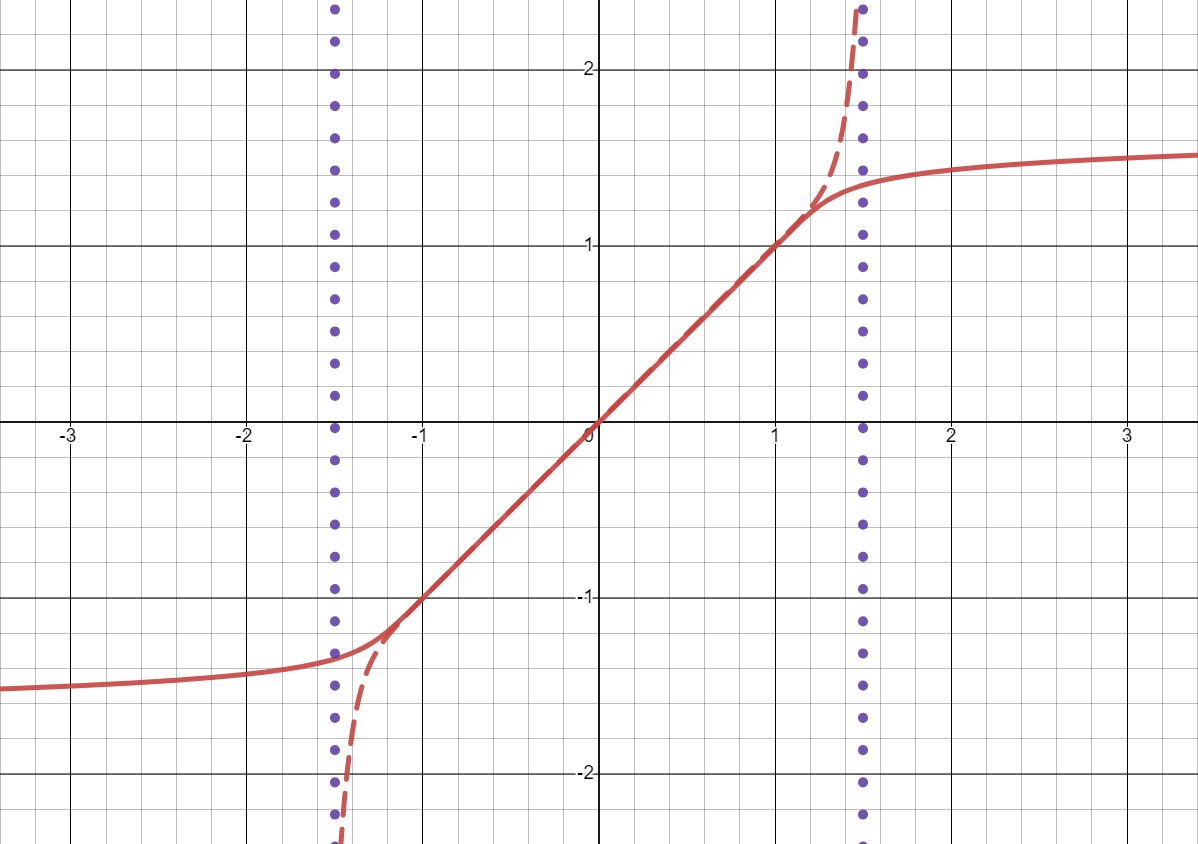
\includegraphics[width = 0.5\textwidth]{2 - implementation/2 - adding damped backgrounds/images/example damping function.png}
            \caption{$v^{\sf damp} = 1.5$, $k = 20$}
        \end{figure}
    \end{frame}
    
    \begin{frame}{Implementation | Adding Damped Distribution}
        \begin{itemize}
            \item  Damped velocity distribution
        \end{itemize}
        \begin{figure}
            \centering
            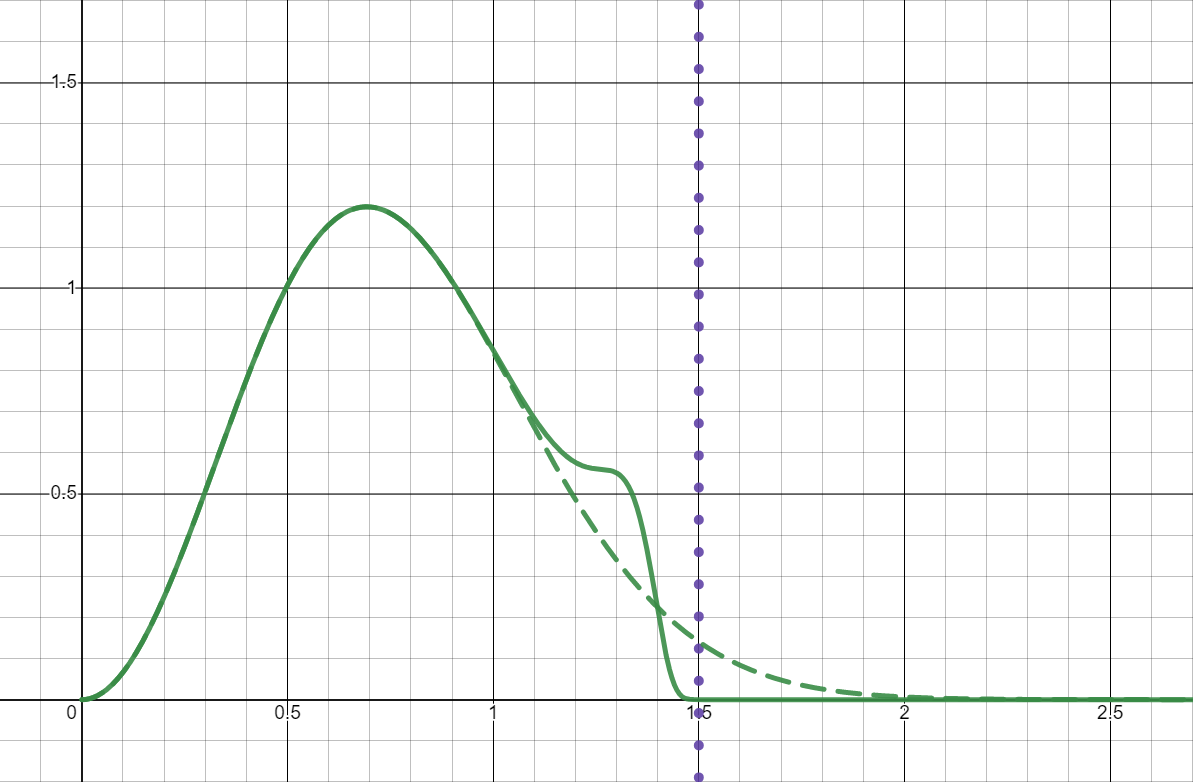
\includegraphics[width = 0.6\textwidth]{2 - implementation/2 - adding damped backgrounds/images/example velocity distribution.png}
            \caption{$v^{\sf damp} = 1.5$, $k = 20$, $u = 0$, $T = 0.48$}
        \end{figure}
    \end{frame}
    
    \begin{frame}{Implementation | Adding Damped Distribution}
        \begin{itemize}
            \item  Damped energy distribution
        \end{itemize}
        \begin{figure}
            \centering
            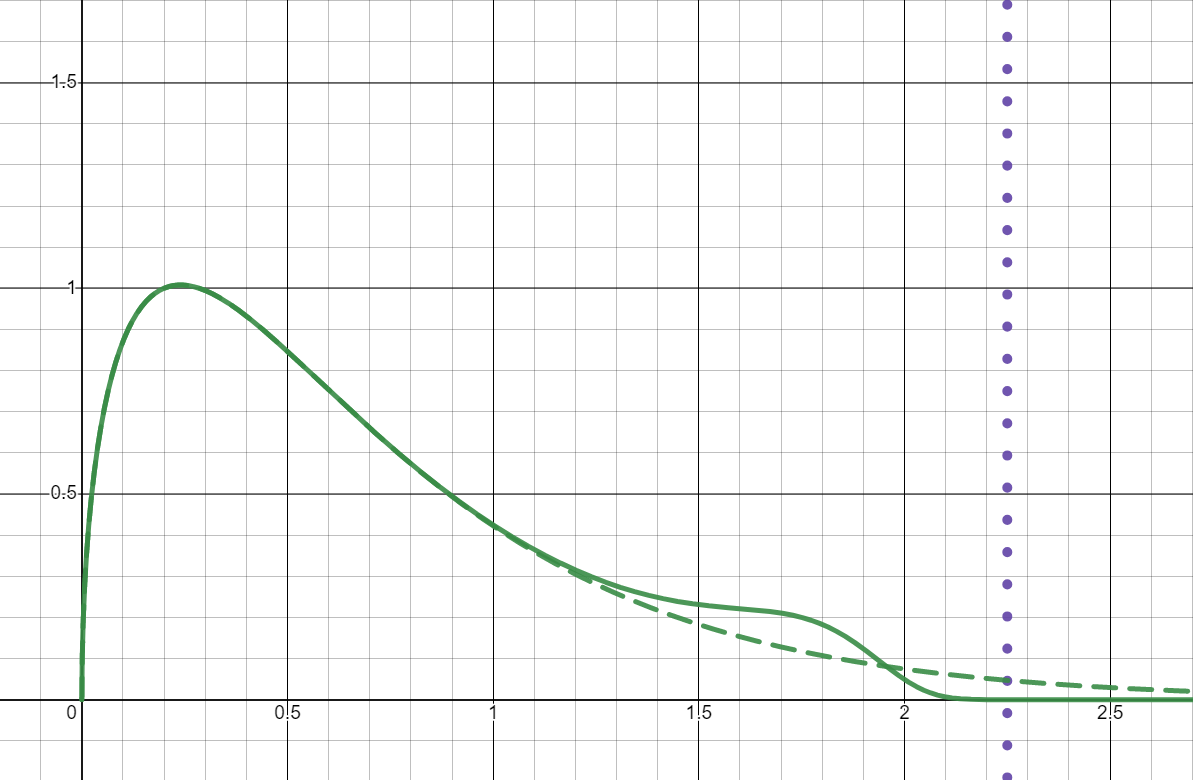
\includegraphics[width = 0.6\textwidth]{2 - implementation/2 - adding damped backgrounds/images/example energy distribution.png}
            \caption{$v^{\sf damp} = 1.5$, $k = 20$, $u = 0$, $T = 0.48$}
        \end{figure}
    \end{frame}
    
    \begin{frame}{Background and Motivation}    
        \begin{figure}
            \centering
            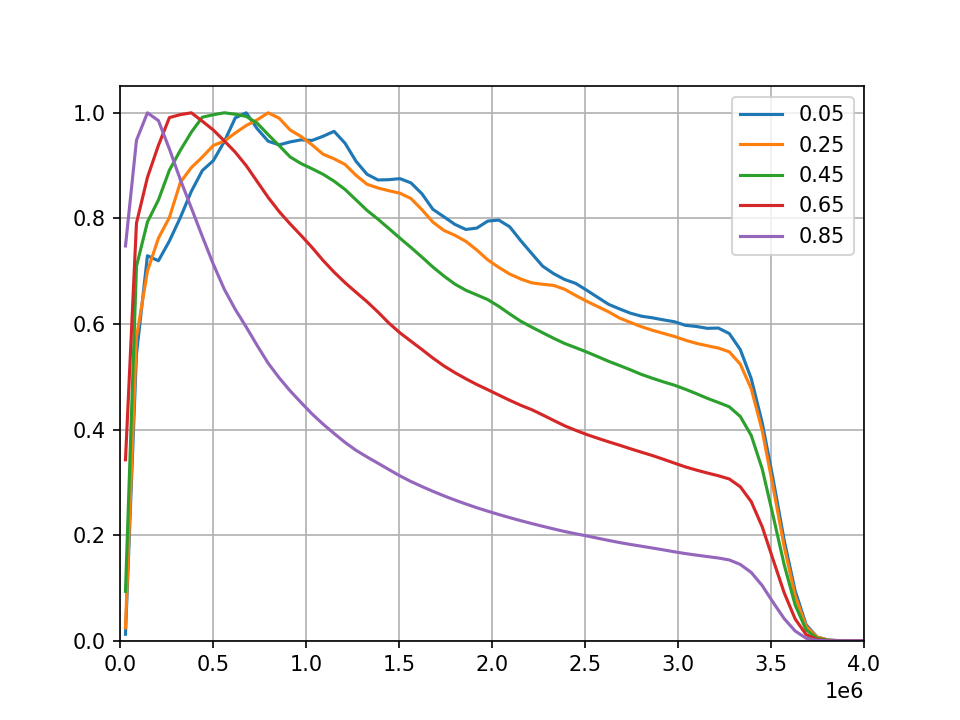
\includegraphics[width = 0.65\textwidth]{1 - background and motivation/images/Experimental Damped Distributions.png}
            \caption{Energy density profiles (on different flux tubes) showing the damping of (alpha) particles over a certain threshold energy(/velocity)}
        \end{figure}
    \end{frame}
    
    \begin{frame}{Implementation | Adding Damped Distribution}
        \begin{itemize}
            \item  Damped \emph{shifted} velocity distribution
        \end{itemize}
        \begin{figure}
            \centering
            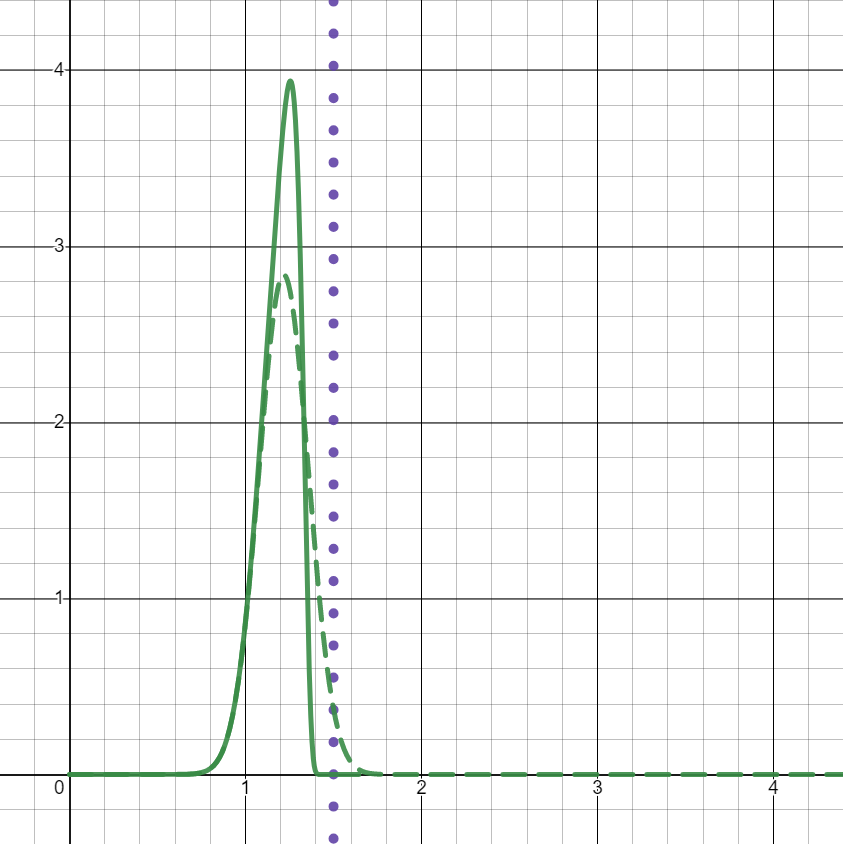
\includegraphics[width = 0.4\textwidth]{2 - implementation/2 - adding damped backgrounds/images/example shifted velocity distribution.png}
            \caption{$v^{\sf damp} = 1.5$, $k = 20$, $u = 1.2$, $T = 0.04$}
        \end{figure}
    \end{frame}
    
    \begin{frame}{Implementation | Adding Damped Distribution}
        \begin{itemize}
            \item  Damped \emph{shifted} energy distribution
        \end{itemize}
        \begin{figure}
            \centering
            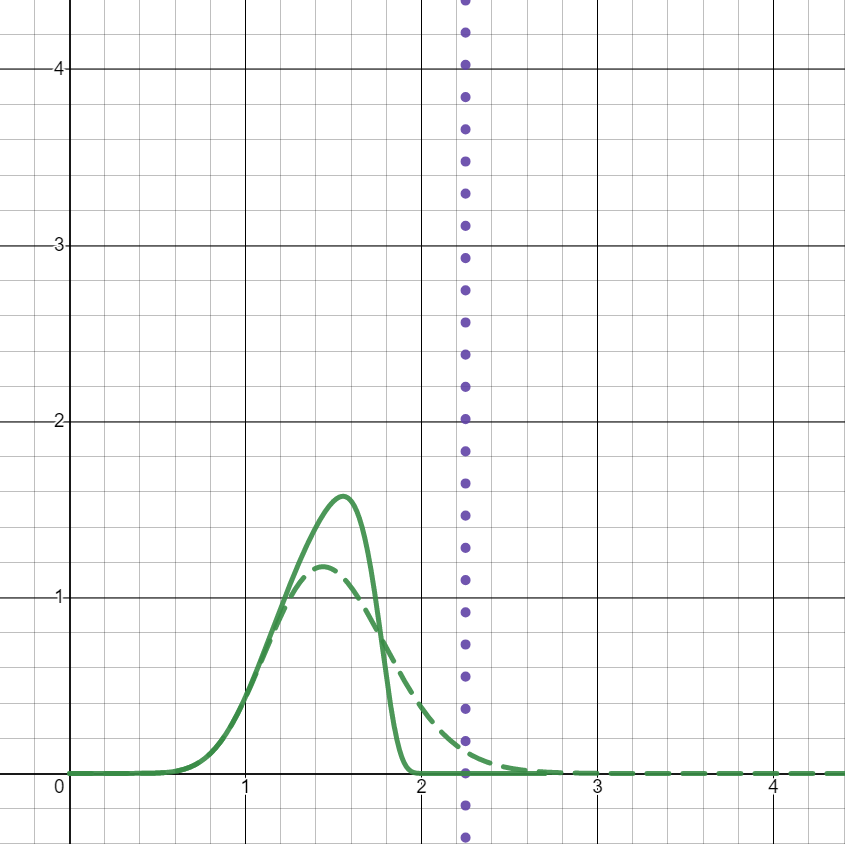
\includegraphics[width = 0.4\textwidth]{2 - implementation/2 - adding damped backgrounds/images/example shifted energy distribution.png}
            \caption{$v^{\sf damp} = 1.5$, $k = 20$, $u = 1.2$, $T = 0.04$}
        \end{figure}
    \end{frame}
    
    \begin{frame}{Implementation | Adding Damped Distribution}
        \vspace{4mm}
        .{\bf HOW DO WE IMPLEMENT THIS IN FULL GENERALITY?}  \pause
        \vspace{2mm}
        
        \begin{figure}[!h]
    \centering
    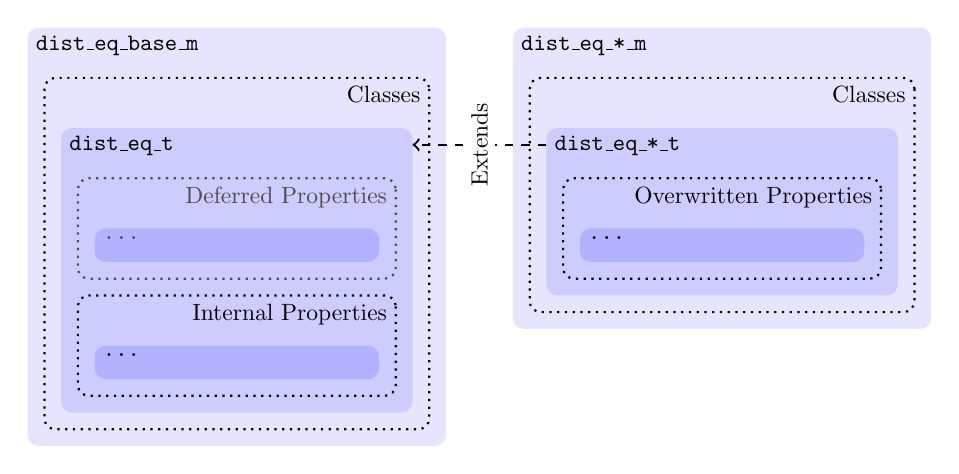
\begin{tikzpicture}[scale = 0.85, every node/.style = {scale = 0.85}, every text node part/.style = {align = left}]
        \fill[rounded corners, fill = blue!10]
            (0, 0) node[below right] {\tt dist\_eq\_base\_m}
            rectangle
            (6.25, -6.25);
            \draw[rounded corners, dotted, thick]
                (6, -0.75) node[below left] {Classes}
                rectangle
                (0.25, -6);
                \fill[rounded corners, fill = blue!20]
                    (0.5, -1.5) node[below right] {\tt dist\_eq\_t}
                    rectangle
                    (5.75, -5.75);
                    \draw[rounded corners, dotted, thick, dotted, black!70]
                        (5.5, -2.25) node[below left] {Deferred Properties}
                        rectangle
                        (0.75, -3.75);
                        \fill[rounded corners, fill = blue!30]
                            (1, -3) node[below right] {}
                            rectangle
                            (5.25, -3.5);
                        \node[black!70] at (1, -3) [below right] {
                                {\tt ...}
                            };
                    \draw[rounded corners, dotted, thick]
                        (5.5, -4) node[below left] {Internal Properties}
                        rectangle
                        (0.75, -5.5);
                        \fill[rounded corners, fill = blue!30]
                            (1, -4.75) node[below right] {}
                            rectangle
                            (5.25, -5.25);
                        \node at (1, -4.75) [below right] {
                                {\tt ...}
                            };
        \fill[rounded corners, fill = blue!10]
            (7.25, 0) node[below right] {\tt dist\_eq\_*\_m}
            rectangle
            (13.5, -4.5);
            \draw[rounded corners, dotted, thick]
                (13.25, -0.75) node[below left] {Classes}
                rectangle
                (7.5, -4.25);
                \fill[rounded corners, fill = blue!20]
                    (7.75, -1.5) node[below right] {\tt dist\_eq\_*\_t}
                    rectangle
                    (13, -4);
                    \draw[rounded corners, dotted, thick]
                        (12.75, -2.25) node[below left] {Overwritten Properties}
                        rectangle
                        (8, -3.75);
                        \fill[rounded corners, fill = blue!30]
                            (8.25, -3) node[below right] {}
                            rectangle
                            (12.5, -3.5);
                        \node at (8.25, -3) [below right] {
                                {\tt ...}
                            };
        \draw[->, thick, dashed]
            (7.75, -1.75) -- (5.75, -1.75)
            node[midway, rotate = 90, fill = white] {Extends};
    \end{tikzpicture}
\end{figure}
    \end{frame}
    
    \begin{frame}{Implementation | Adding Damped Distribution}
        \begin{itemize}
            \item  What kind of functionals does the {\tt dist\_eq\_*\_damped\_t} class instance need to evaluate?
            \begin{center}\begin{tabular}{ c | c }
                Procedure  &  Functional  \\
                \hline\hline
                {\tt get\_*D\_dv}  &  $\partial_{v_{\parallel}}f_{s0}$  \\
                \hline
                {\tt get\_*D\_dm}  &  $\partial_{\mu}f_{s0}$  \\
                \hline
                {\tt get\_*D\_dvdm}  &  $\frac{B_{0}}{2}\partial_{v_{\parallel}}f_{s0} - v_{\parallel}\partial_{\mu}f_{s0}$  \\
                \hline
                \vdots  &  \vdots  \\
            \end{tabular}\end{center}  \pause

            \item  Needs access to:
            \begin{itemize}
                \item  $v_{\parallel}^{\sf pre}$, $\mu^{\sf pre}$ (and their derivatives up to 2nd order)
                \item  $J$ (and its derivative up to 1st order)
            \end{itemize}
        \end{itemize}
    \end{frame}
    
    \begin{frame}{Implementation | Adding Damped Distribution}
        \vspace{2mm}
        \begin{figure}[!h]
    \centering
    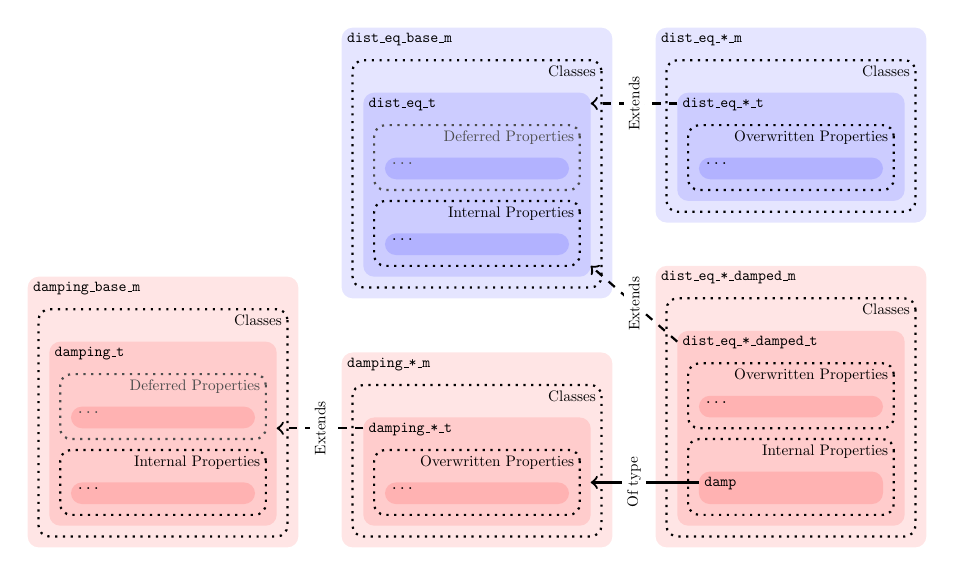
\begin{tikzpicture}[scale = 0.55, every node/.style = {scale = 0.55}, every text node part/.style = {align = left}]
        \fill[rounded corners, fill = blue!10]
            (0, 0) node[below right] {\tt dist\_eq\_base\_m}
            rectangle
            (6.25, -6.25);
            \draw[rounded corners, dotted, thick]
                (6, -0.75) node[below left] {Classes}
                rectangle
                (0.25, -6);
                \fill[rounded corners, fill = blue!20]
                    (0.5, -1.5) node[below right] {\tt dist\_eq\_t}
                    rectangle
                    (5.75, -5.75);
                    \draw[rounded corners, dotted, thick, dotted, black!70]
                        (5.5, -2.25) node[below left] {Deferred Properties}
                        rectangle
                        (0.75, -3.75);
                        \fill[rounded corners, fill = blue!30]
                            (1, -3) node[below right] {}
                            rectangle
                            (5.25, -3.5);
                        \node[black!70] at (1, -3) [below right] {
                                {\tt ...}
                            };
                    \draw[rounded corners, dotted, thick]
                        (5.5, -4) node[below left] {Internal Properties}
                        rectangle
                        (0.75, -5.5);
                        \fill[rounded corners, fill = blue!30]
                            (1, -4.75) node[below right] {}
                            rectangle
                            (5.25, -5.25);
                        \node at (1, -4.75) [below right] {
                                {\tt ...}
                            };
        \fill[rounded corners, fill = blue!10]
            (7.25, 0) node[below right] {\tt dist\_eq\_*\_m}
            rectangle
            (13.5, -4.5);
            \draw[rounded corners, dotted, thick]
                (13.25, -0.75) node[below left] {Classes}
                rectangle
                (7.5, -4.25);
                \fill[rounded corners, fill = blue!20]
                    (7.75, -1.5) node[below right] {\tt dist\_eq\_*\_t}
                    rectangle
                    (13, -4);
                    \draw[rounded corners, dotted, thick]
                        (12.75, -2.25) node[below left] {Overwritten Properties}
                        rectangle
                        (8, -3.75);
                        \fill[rounded corners, fill = blue!30]
                            (8.25, -3) node[below right] {}
                            rectangle
                            (12.5, -3.5);
                        \node at (8.25, -3) [below right] {
                                {\tt ...}
                            };
        \fill[rounded corners, fill = red!10]
            (-7.25, -5.75) node[below right] {\tt damping\_base\_m}
            rectangle
            (-1, -12);
            \draw[rounded corners, dotted, thick]
                (-1.25, -6.5) node[below left] {Classes}
                rectangle
                (-7, -11.75);
                \fill[rounded corners, fill = red!20]
                    (-6.75, -7.25) node[below right] {\tt damping\_t}
                    rectangle
                    (-1.5, -11.5);
                    \draw[rounded corners, dotted, thick, dotted, black!70]
                        (-1.75, -8) node[below left] {Deferred Properties}
                        rectangle
                        (-6.5, -9.5);
                        \fill[rounded corners, fill = red!30]
                            (-6.25, -8.75) node[below right] {}
                            rectangle
                            (-2, -9.25);
                        \node[black!70] at (-6.25, -8.75) [below right] {
                                {\tt ...}
                            };
                    \draw[rounded corners, dotted, thick]
                        (-1.75, -9.75) node[below left] {Internal Properties}
                        rectangle
                        (-6.5, -11.25);
                        \fill[rounded corners, fill = red!30]
                            (-6.25, -10.5) node[below right] {}
                            rectangle
                            (-2, -11);
                        \node at (-6.25, -10.5) [below right] {
                                {\tt ...}
                            };
        \fill[rounded corners, fill = red!10]
            (0, -7.5) node[below right] {\tt damping\_*\_m}
            rectangle
            (6.25, -12);
            \draw[rounded corners, dotted, thick]
                (6, -8.25) node[below left] {Classes}
                rectangle
                (0.25, -11.75);
                \fill[rounded corners, fill = red!20]
                    (0.5, -9) node[below right] {\tt damping\_*\_t}
                    rectangle
                    (5.75, -11.5);
                    \draw[rounded corners, dotted, thick]
                        (5.5, -9.75) node[below left] {Overwritten Properties}
                        rectangle
                        (0.75, -11.25);
                        \fill[rounded corners, fill = red!30]
                            (1, -10.5) node[below right] {}
                            rectangle
                            (5.25, -11);
                        \node at (1, -10.5) [below right] {
                                {\tt ...}
                            };
        \fill[rounded corners, fill = red!10]
            (7.25, -5.5) node[below right] {\tt dist\_eq\_*\_damped\_m}
            rectangle
            (13.5, -12);
            \draw[rounded corners, dotted, thick]
                (13.25, -6.25) node[below left] {Classes}
                rectangle
                (7.5, -11.75);
                \fill[rounded corners, fill = red!20]
                    (7.75, -7) node[below right] {\tt dist\_eq\_*\_damped\_t}
                    rectangle
                    (13, -11.5);
                    \draw[rounded corners, dotted, thick]
                        (12.75, -7.75) node[below left] {Overwritten Properties}
                        rectangle
                        (8, -9.25);
                        \fill[rounded corners, fill = red!30]
                            (8.25, -8.5) node[below right] {}
                            rectangle
                            (12.5, -9);
                        \node at (8.25, -8.5) [below right] {
                                {\tt ...}
                            };
                    \draw[rounded corners, dotted, thick]
                        (12.75, -9.5) node[below left] {Internal Properties}
                        rectangle
                        (8, -11.25);
                        \fill[rounded corners, fill = red!30]
                            (8.25, -10.25) node[below right] {}
                            rectangle
                            (12.5, -11);
                        \node at (8.25, -10.25) [below right] {
                                {\tt damp}
                            };
        \draw[->, thick, dashed]
            (7.75, -1.75) -- (5.75, -1.75)
            node[midway, rotate = 90, fill = white] {Extends};
        \draw[->, thick, dashed]
            (7.75, -7.25) -- (5.75, -5.5)
            node[midway, rotate = 90, fill = white] {Extends};
        \draw[->, thick, dashed]
            (0.5, -9.25) -- (-1.5, -9.25)
            node[midway, rotate = 90, fill = white] {Extends};
        \draw[->, thick]
            (8.25, -10.5) -- (5.75, -10.5);
            \node[rotate = 90, fill = white] at (6.75, -10.5) {Of type};
    \end{tikzpicture}
\end{figure}
    \end{frame}
    
    \begin{frame}{Implementation | Adding Damped Distribution}
        .{\bf CODE NOW AVAILABLE!}
        In my Gitlab repository:
        \begin{itemize}
            \item  Just ask me for access! :)
            \item  \underline{https://gitlab.mpcdf.mpg.de/g-borisandrews/gene-gpu}
            \begin{center}
                
\includegraphics[width = 0.3\textwidth]{2 - implementation/2 - adding damped backgrounds/images/QR.png}
            \end{center}
            \item  Also have a far more detailed report to which Salomon should have access
        \end{itemize}
    \end{frame}
    